\section{第三章\quad 气体和蒸汽的性质}
\pt{理想气体}假设分子为不占体积的弹性质点，认为除碰撞外分子间无作用力，是实际气体在\pt{低压高温的抽象}，主要是\pt{低压}

\pt{理想气体状态方程}

$$
    \left\{
    \begin{aligned}
         & pV=mR_{\mathrm{g}}T &  & \text{质量为} m      \\
         & pv=R_{\mathrm{g}}T  &  & 1\,\mathrm{kg} 气体 \\
         & pV=nRT              &  & \text{物质的量为} n
    \end{aligned}
    \right.
$$

$R=8.3145\,\mathrm{J/(mol\cdot K)}$

\divider

\pt{比热容} $\displaystyle c=\lim_{\Delta T\to 0}\frac{q}{\Delta T}=\frac{\delta q}{\mathrm{d}T}$，通常是温度的函数，并且与过程相关

$$
    c=\frac{\partial u}{\partial T}+\left(\frac{\partial u}{\partial v}+p\right)\frac{\mathrm{d}v}{\mathrm{d}T}
$$

\pt{定压比热容} $\displaystyle c_V=\frac{\mathrm{d}h}{\mathrm{d}T}$，
\pt{定容比热容} $\displaystyle c_p=\frac{\mathrm{d}u}{\mathrm{d}T}$，
\pt{迈耶公式} $c_p-c_V=R_\mathrm{g}$，
\pt{比热容比} $\displaystyle \gamma = \frac{c_p}{c_v}$，$\displaystyle c_p=\frac{\gamma R_\mathrm{g}}{\gamma -1}$，$\displaystyle c_V=\frac{R_\mathrm{g}}{\gamma -1}$

\divider

\tdo{水的 $c_p$ 和 $c_v$ 关系，ppt 18 页，待定}

\divider

使用比热容计算热量的途径

\pt{积分计算} $q = \int_{T_1}^{T_2} c\ \mathrm{d}T$，
\pt{平均比热容表} $q=\int_0^{T_2} c\ \mathrm{d}T - \int_0^{T_1} c\ \mathrm{d}T = c_n\vert_0^{T_2}\cdot T_2-c_n\vert_0^{T_1}\cdot T_1$，
\pt{平均比热直线式}：令 $c_n= a + bT$，则 $q = \int_{T_1}^{T_2} (a + bT)\ \mathrm{d}T = a(T_2-T_1)+\frac{b}{2}(T_2^2-T_1^2) = \left(a + \frac{b}{2}(T_1+T_2)\right)(T_2-T_1)$，平均比热容为 $c\vert_{n,t_1}^{t_2}=a+\frac{b}{2}(t_1+t_2)$，
\pt{定值比热容}认为比热容为常数，$q = c(T_2-T_1)$ 根据气体分子运动理论，$C_{V,\mathrm{m}}=\frac{i}{2}R$，$C_{p,\mathrm{m}}=\frac{i+2}{2}R$，$\gamma=\frac{i+2}{i}$，单、双、多原子分子的 $i$ 分别为 $3$ 、$5$ 和 $6$

\divider

\pt{理想气体的热力学能} $\mathrm{d}u = c_V\,\mathrm{d}T$，焓 $\mathrm{d}h = c_p\,\mathrm{d}T$，内能和焓仅是温度的函数，变化量与路径无关。对于\pt{P可逆过程}，理想气体的\pt{熵} $\mathrm{d}s = \frac{\delta q_\mathrm{rev}}{T}=c_V\frac{\mathrm{d}T}{T}+R_{\mathrm{g}}\frac{\mathrm{d}v}{v}$，$\Delta s=\int_{T_1}^{T_2}c_V\frac{\mathrm{d}T}{T}+R_{\mathrm{g}}\ln\frac{v_2}{v_1}=c_V\ln\frac{T_2}{T_1}+R_{\mathrm{g}}\ln\frac{v_2}{v_1}=\int_{T_1}^{T_2}c_p\frac{\mathrm{d}T}{T}-R_{\mathrm{g}}\ln\frac{p_2}{p_1}=c_p\ln\frac{T_2}{T_1}-R_{\mathrm{g}}\ln\frac{p_2}{p_1}$

\divider

\pt{汽化}：液态变为气态的过程；\pt{蒸发}：发生在液体表面的汽化过程；\pt{沸腾}：在液体表面和内部同时进行的剧烈汽化过程；\pt{液化}：气相变为液相的过程。\pt{饱和状态}：气化速度 $=$ 液化速度，宏观上气液两相保持一定的相对数量。饱和温度 $t_s$ 和饱和压力 $p_s$ 一一对应

\pt{饱和液}：处于饱和状态的液体，$t=t_s$；
\pt{干饱和蒸汽}：处于饱和状态的蒸汽，$t=t_s$；
\pt{未饱和液}：温度低于该压力下饱和温度的液体，$t<t_s$；
\pt{过热蒸汽}：温度高于饱和温度的蒸汽，$t>t_s$；
\pt{过热度}：$d=t-t_s$。
使得未饱和液变成饱和液的方法有：保持压力不变升高温度；保持温度不变降低压力。\pt{干度}：湿蒸汽中干饱和蒸汽的质量分数 $x=\frac{m_v}{m_v+m_l}$；
\pt{湿度}：$y=1-x$；
\pt{三相点}：气、液、固三相平衡共存的状态

\divider

水定压加热气化过程：
\pt{预热}：未饱和水升温到饱和水；
\pt{气化}：饱和水变为干饱和蒸汽；
\pt{过热}：干饱和蒸汽继续升温变为过热蒸汽

定压加热过程中的典型状态：
\pt{未饱和水}：$t<t_s$；\pt{饱和水}：$t=t_s$，开始汽化；\pt{湿蒸汽}：$t=t_s$，液、汽共存；\pt{干饱和蒸汽}：$x=1$，汽化结束；\pt{过热蒸汽}：$t>t_s$。

\noindent
\begin{minipage}[t]{0.48\linewidth}
    \vspace{0pt}
    \centering
    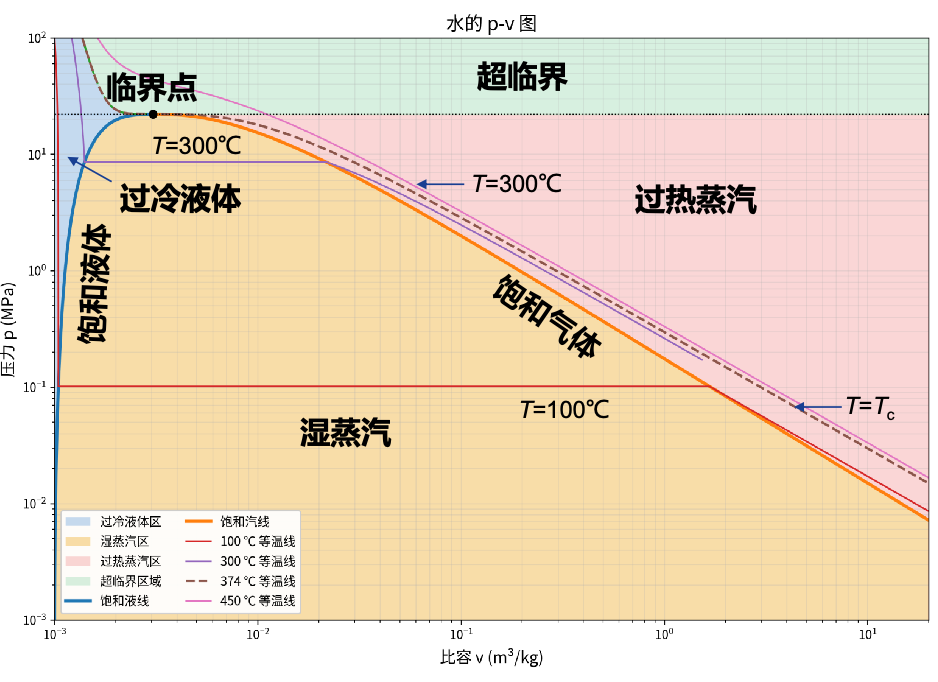
\includegraphics[width=\linewidth]{figures/3水pv图.png}
\end{minipage}
\hfill
\begin{minipage}[t]{0.48\linewidth}
    \vspace{0pt}
    \centering
    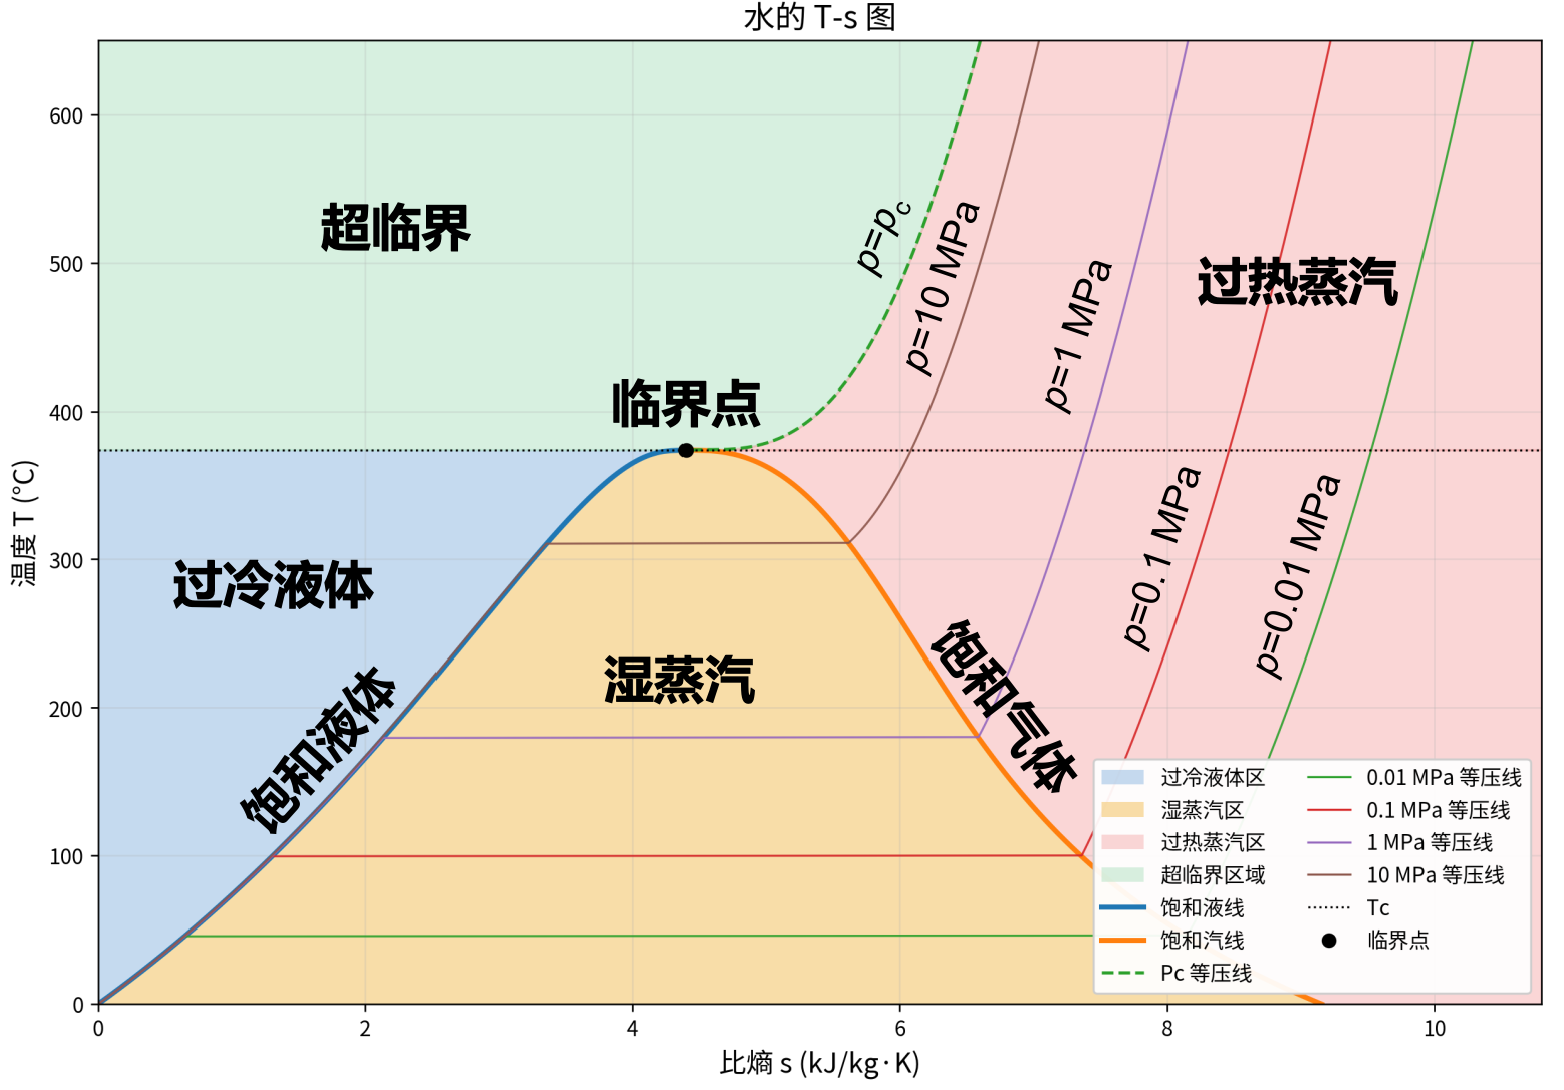
\includegraphics[width=\linewidth]{figures/3水Ts图.png}
\end{minipage}

\divider

动力工程中水蒸气不能用理性想气体性质计算。
规定三相点液态水热力学能和熵为 $0$，$u^\prime_{273.16}=0$，$s^\prime_{273.16}=0$，焓近似为 $0$。

\pt{未饱和水} $(t,p)$ ：查图标或者由专用程序计算得到，压力不太高时近似 $h_t = c_p t$，$s_t=c_p\ln\frac{T}{273.16}$

\pt{饱和水和饱和水蒸气} $p_s$ 或 $t_s$：查表或者程序算

\pt{过热蒸汽} $(p_t)$：查表或者程序算，不能用类似未饱和水的简单近似式

\pt{湿饱和蒸汽} $t_s$ （或 $p_s$）和 $x$：
\pt{比体积} $v_x=xv^{\prime\prime}+(1-x)v^\prime=v^\prime+x(v^{\prime\prime}-v^\prime)$，当 $x$ 较大时 $v_x\approx xv^{\prime\prime}$；
\pt{焓} $h_x=xh^{\prime\prime}+(1-x)h^\prime=h\prime+x(h^{\prime\prime}-h^\prime)$，
$\gamma = h^{\prime\prime}-h^\prime$ 为汽化潜热，可用 $gamma$ 将焓化为 $h_x=h^\prime+x\gamma$，$s_x=xs^{\prime\prime}+(1-x)s^\prime=s^\prime+x(s^{\prime\prime}-s^\prime)$；
\pt{熵}：$s_x=xs^{\prime\prime}+(1-x)s^\prime=s^\prime+x(s^{\prime\prime}-s^\prime)$，饱和相变中 $s^{\prime\prime}-s^\prime=\frac{\gamma}{T_s}$，则 $s_x=s^\prime+x\frac{\gamma}{T_s}$；
\pt{热力学能}：$u_x=h_x-p_sv_x$

\divider